\section{A Series of Tubes - A Tool for Pipe Design}

To allow makers to design novel objects with pipe-powered interfaces, we created a tool for use on arbitrary 3D models.  This tool allows designers to select exterior connection points of their pipes (see Figure \ref{fig:tool-process-interior}) or to import vector art describing the pipes' interior paths (see Figure \ref{fig:tool-process-exterior}).  Once the maker's selections are made, we create a complete routing using either the exterior connection point method (A*, physical simulation) or the interior path method (graph edge creation, Euler circuit generation).  We thicken our routing to create pipes. \valkyrie{We also apply templates where appropriate (e.g., 3D cross-overs for tubes that intersect in the plane).}  The resultant pipes are subtracted from the original mesh, which can then be 3D printed.

Our tool is implemented as a part of Meshmixer, a consumer 3D mesh editing tool, in C++.

\subsection{Exterior Connection Points}

Designing objects which, for example, are touch sensitive in particular areas or need to integrate with existing electronics, requires precise location and sizing of pipe endpoints.  The interior of these pipes should have as large a bending radius as possible so that post-print insertion of solid or viscous media (like wire or paint) is easier.

To create pipes in which the location and shape of exterior connection points matters, we first allow makers to select the connection points on the mesh's surface using a brush. Our tool then creates an initial shortest-path routing using A* to estimate the routed distance between points.  This routing is used to create a rod; we run physics-based simulation steps on the rod to minimize its bending energy (and thereby minimize the bend radius of the tubes).

\begin{figure}[h!]
\centering
    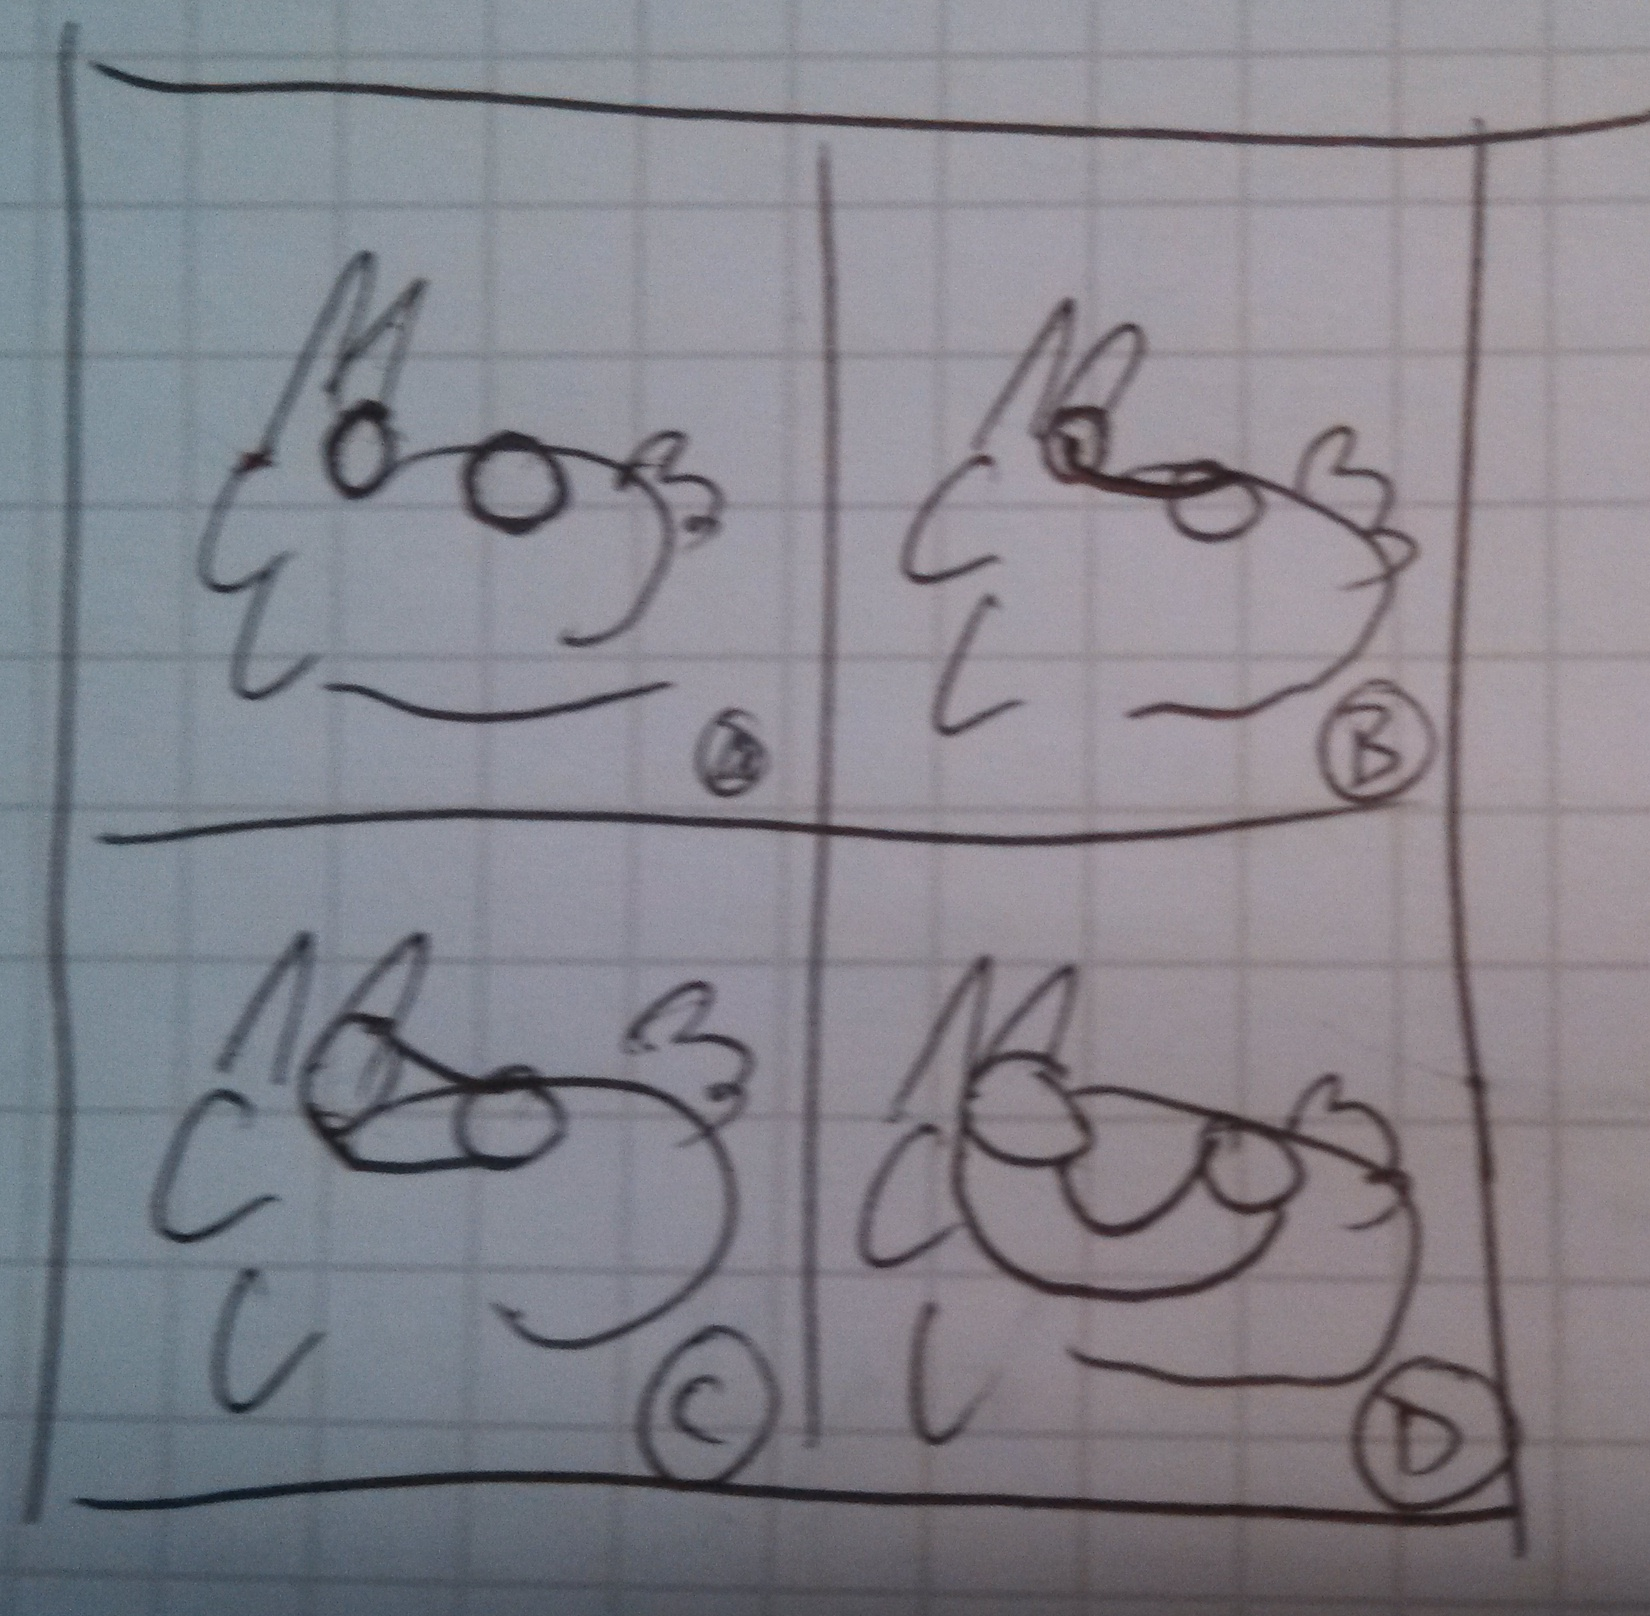
\includegraphics[width=3.4in]{figures/placeholder/exterior.jpg}
\caption{An example mesh with exterior connection points selected.  The initial A* routing is drawn in {\color{red}red}, and in {\color{tovi}green} is our physically-based rod after simulation.}
\label{fig:tool-process-exterior}
\end{figure}

\subsubsection{Routing and Physical Simulation}

Our basic first-pass routing algorithm uses the A* routing algorithm \cite{Hart-Astar}.  The path cost in our implementation is based only on shortest distance between the starting and ending points, without weighting for distance from the surface.  We only permit the routing within the voxel grid of the mesh: i.e., the routing is not permitted to traverse through space outside the mesh itself.

Given this initial routing, we create a rod of slightly longer proportional length.  The rod must be longer, as the A* routing can follow the mesh boundaries and the rod requires extra length to be pushed away from the mesh surface.  While we do not have a theoretical basis for this proportional increase, \valkyrie{yet.  what might it be related to?  we can test how much of the A* path is outside the model, and how much is inside; further we can consider the distance from the A* path that is outside the model to the surface.  I think there's a good way to do this.  It might even just mean iteratively changing the rod length until we get something reasonably short and also smooth.  we can also return to the A* that I wrote which finds a routing through the mesh that respects its boundaries; this would get us closer to what we need for length in the first place.}, we have found 1.15 to be a reasonable multiplier in practice.  A too-long rod is forced to kink and expand further than necessary inside the model, while a too-short rod must be stretched, leading to non-smooth bending.

To allow for easiest insertion of media post-print, our physical simulation step minimizes the bend radius of the generated rods.  In order to force our simulated rods away from the surface of the mesh, we create ``wind'' pushing inward from the exterior of the mesh.  This wind keeps the resulting pipe away from the surface. \valkyrie{Ryan: How does it actually work?}

\subsubsection{Pipes with Multiple Endpoints}
For the creation of pipes with multiple endpoints, for example the star topologies in Figure \ref{fig:toys} or tree topologies, makers can select interior faces of existing pipes as endpoints, and thereby create pipe networks by hand.  We do not currently offer any pipe network manipulation tools.

\valkyrie{To allow designers to create pipes with multiple endpoints (like the star topologies in Figure \ref{fig:toys}), we create 0-size mesh points in the center of the object, to which we attach one end of every pipe?}

\subsubsection{Pipes with Non-Round Endpoints}
Our tool does not explicitly allow makers to design the shape of their pipes' endpoints.  However, the larger Meshmixer package does allow brushing arbitrary shapes onto the surface and extruding them inward, as in Figure \ref{fig:meshmixer-endpoint}.

\subsubsection{Semi-Closed and Fully Enclosed Pipes}
Users can select via a checkbox if they wish to cap one end, the other end, or both ends of their pipe.  The software simply creates an offset from the surface in these cases, so that material remains between the pipe and the surface after mesh modification.

\begin{figure}[h!]
\centering
    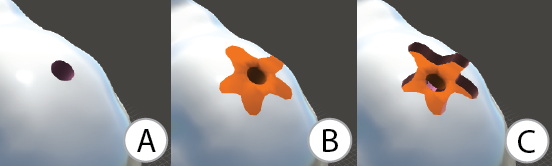
\includegraphics[width=3.4in]{figures/meshmixer-endpoint.png}
\caption{After creating a tube, a maker can select a surface shape using a brush (a).  She can then extrude her selection inward (b).}
\label{fig:meshmixer-endpoint}
\end{figure}

\subsection{Designing Interior Paths}

Neon signs, as in Figure \ref{fig:tool-process-interior}(d), require a single long path that passes through many desired edges: for example, in our UIST sign, the path must pass through all the edges that comprise the word ``UIST''.  To allow makers to create novel neon signs, as well as similar objects that require design of the pipe's interior path, we built a tool which leverages graph theory to generate this single long path.

A maker can import a vector graphics file (such as SVG) describing the path she desires for her pipes.  We create a graph based on this input data, then add edges to make it connected and semi-Eulerian.  We create an Euler tour on the modified graph, and thicken the path to create pipes.  \valkyrie{3D templates are used to resolve tube crossings in the plane.}  We cut these pipes from a generated block mesh large enough to hold them.

\begin{figure}[h!]
\centering
    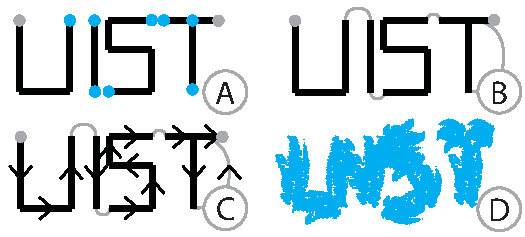
\includegraphics[width=3.4in]{figures/interior.pdf}
\caption{An input vector graphics file with the points which cannot be tubed as drawn highlighted in {\color{blue}blue} (a).  The connected graph created by our software (b) and the resulting Euler circuit (c) permit creation of a novel neon sign (d).}
\label{fig:tool-process-interior}
\end{figure}

\subsubsection{Routing}
The interior path routing problem is a version of the Chinese Postman Problem\footnote{The CPP is also known as the route inspection problem: \url{http://en.wikipedia.org/wiki/Route_inspection_problem}}, in which we wish to traverse all edges of the graph described in the user's input with a single Euler circuit, much as a postman needs to walk along every road at least once to deliver mail.  We call our relaxation the Spiderman Postman Problem: we allow the creation of non-existing paths (i.e., the postman may traverse buildings in addition to roads).  If inputted path components are disconnected, we must create edges that connect them; additionally we can create new edges connecting odd-degree vertices rather than simply retracing existing edges.  In the final artifact, all created edges will be blocked out by dark material so the inserted medium is not visible (see Figure \ref{fig:tool-process-interior}).  We offer a short algorithm here, with a more mathematically precise definition and associated proof in the appendix.

We need a graph which is semi-Eulerian (i.e., the inserted media can enter at one point, traverse every edge exactly once, and exit at a different point).  In order to create a semi-Eulerian graph, we first add a temporary edge to the start and end points.  This is removed after the graph is made fully Eulerian.

In order to connect disconnected subgraphs in the input, we reduce each disconnected subgraph to a point.  We add edges from each subgraph-point to each other subgraph-point that represent the minimum distance between any two points in the expanded subgraphs (where distance is Euclidean distance).  We greedily select the smallest weight edges until all subgraphs are joined into a single graph.  We re-expand the subgraphs.

In order to make our graph Eulerian, we consider all vertices of odd degree in the connected graph and make a clique of edges once more based on distance.  We again greedily select edges between the odd nodes until no odd nodes remain.  Finally, we remove our temporary edge, which changes the graph from Eulerian to semi-Eulerian.  This graph is a connected, semi-Eulerian graph which contains all edges in the input SVG (see Appendix).

We believe that a lower total weight matching is possible by connecting components and ensuring edge degree evenness together in a global process, however it this not crucial for our purposes.

Once we have a semi-Eulerian graph, we need to create an Euler tour.  An Euler tour is a path that touches every edge once, beginning and ending at the two nodes of odd degree: in this case, those are the user-selected start and end nodes.  We use a weighted modification of Fleury's algorithm\footnote{\url{http://en.wikipedia.org/wiki/Eulerian_path\#Fleury.27s_algorithm}} for this, where instead of randomly selecting from non-bridge paths at each node, we select the path which turns the least from the most recent path (i.e., we prefer to pass straight through a node, if possible).  This minimizes turns in the final artifact, which eases support material removal and assembly.

\begin{figure}[h!]
\centering
    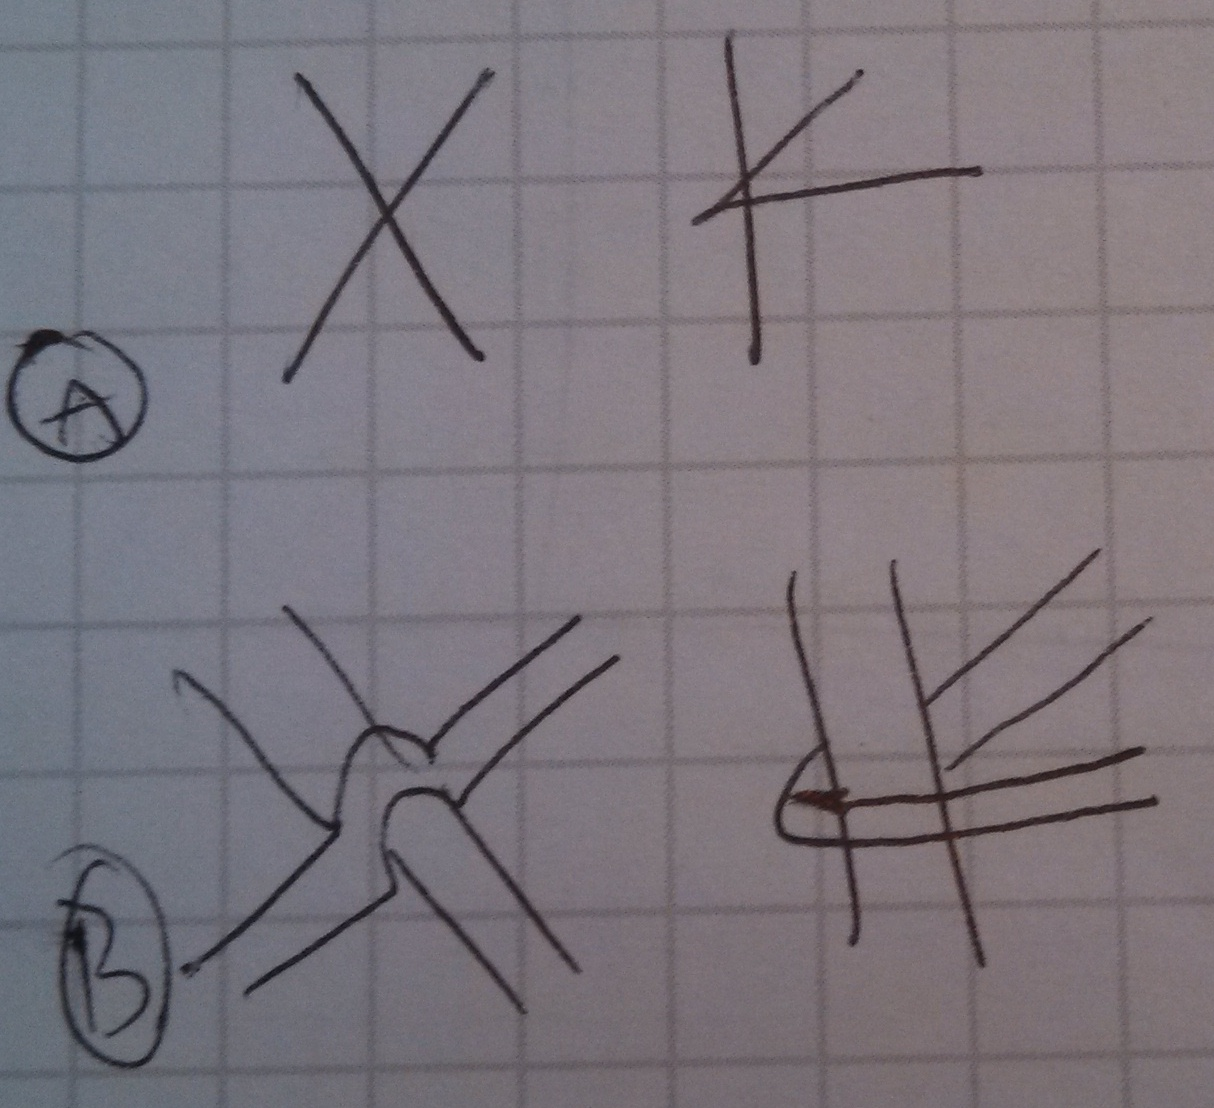
\includegraphics[width=3.4in]{figures/placeholder/templates.jpg}
\caption{\valkyrie{When edges intersect in the plane (a), we match them to the nearest of our several intersection templates (b) to create 3D paths that do not interfere with each other.}}
\label{fig:templates}
\end{figure}

\subsubsection{Edges that Intersect in the Plane}
We do not currently redirect edges that intersect in the plane.  Because we have a 3-dimensional canvas in which to work, it would be possible to push overlapping paths into the third dimension, however the angel hair EL wire we have used for our prototypes is so thin as to make this unnecessary.

\valkyrie{Once we have a tour, we must resolve tubes that intersect in the plane.  Because we have a 3-dimensional canvas in which to work, we can push overlapping paths into the third dimension.

To detect intersecting edges, we \valkyrie{I'm not sure what we do.}.  We also consider edges at nodes with degree $>2$, as these edges are considered to cross.  When intersections have been detected, we match one of several templates to the affected edges (see Figure \ref{fig:templates}) using a nearest neighbors technique.  Our templates are parameterized, so the templates can be modified to accommodate precise intersection characteristics.}

\subsection{Mesh Modification}

How we actually cut stuff and make tubes happen. \valkyrie{Ryan?}